%%%%%%%%%%%%%%%%%%%%%%%%%%%%%%%%%%%%%%%%%
% Wenneker Assignment
% LaTeX Template
% Version 2.0 (12/1/2019)
%
% This template originates from:
% http://www.LaTeXTemplates.com
%
% Authors:
% Vel (vel@LaTeXTemplates.com)
% Frits Wenneker
%
% License:
% CC BY-NC-SA 3.0 (http://creativecommons.org/licenses/by-nc-sa/3.0/)
% 
%%%%%%%%%%%%%%%%%%%%%%%%%%%%%%%%%%%%%%%%%

%----------------------------------------------------------------------------------------
%	PACKAGES AND OTHER DOCUMENT CONFIGURATIONS
%----------------------------------------------------------------------------------------

\documentclass[11pt]{scrartcl} % Font size

%%%%%%%%%%%%%%%%%%%%%%%%%%%%%%%%%%%%%%%%%
% Wenneker Assignment
% Structure Specification File
% Version 2.0 (12/1/2019)
%
% This template originates from:
% http://www.LaTeXTemplates.com
%
% Authors:
% Vel (vel@LaTeXTemplates.com)
% Frits Wenneker
%
% License:
% CC BY-NC-SA 3.0 (http://creativecommons.org/licenses/by-nc-sa/3.0/)
% 
%%%%%%%%%%%%%%%%%%%%%%%%%%%%%%%%%%%%%%%%%

%----------------------------------------------------------------------------------------
%	PACKAGES AND OTHER DOCUMENT CONFIGURATIONS
%----------------------------------------------------------------------------------------

\usepackage{amsmath, amsfonts, amsthm} % Math packages

\usepackage{geometry}

\usepackage{listings} % Code listings, with syntax highlighting

\usepackage[french]{babel} % English language hyphenation

\usepackage{graphicx} % Required for inserting images
\graphicspath{{Figures/}{./}} % Specifies where to look for included images (trailing slash required)

\usepackage{booktabs} % Required for better horizontal rules in tables

\usepackage{subcaption} % Required for creating figures with multiple parts (subfigures)

\usepackage{todonotes} % Required for inserting todo notes

\usepackage{array} % Required for customising tables

\usepackage{hyperref} % Required for adding links	and customising them

\numberwithin{equation}{section} % Number equations within sections (i.e. 1.1, 1.2, 2.1, 2.2 instead of 1, 2, 3, 4)
\numberwithin{figure}{section} % Number figures within sections (i.e. 1.1, 1.2, 2.1, 2.2 instead of 1, 2, 3, 4)
\numberwithin{table}{section} % Number tables within sections (i.e. 1.1, 1.2, 2.1, 2.2 instead of 1, 2, 3, 4)

\setlength\parindent{0pt} % Removes all indentation from paragraphs

\usepackage{enumitem} % Required for list customisation
\setlist{noitemsep} % No spacing between list items

%----------------------------------------------------------------------------------------
%	DOCUMENT MARGINS
%----------------------------------------------------------------------------------------

\usepackage{geometry} % Required for adjusting page dimensions and margins

\geometry{
	paper=a4paper, % Paper size, change to letterpaper for US letter size
	top=2.5cm, % Top margin
	bottom=3cm, % Bottom margin
	left=3cm, % Left margin
	right=3cm, % Right margin
	headheight=0.75cm, % Header height
	footskip=1.5cm, % Space from the bottom margin to the baseline of the footer
	headsep=0.75cm, % Space from the top margin to the baseline of the header
	%showframe, % Uncomment to show how the type block is set on the page
}

%----------------------------------------------------------------------------------------
%	FONTS
%----------------------------------------------------------------------------------------

\usepackage[utf8]{inputenc} % Required for inputting international characters
\usepackage[T1]{fontenc} % Use 8-bit encoding

\usepackage{fourier} % Use the Adobe Utopia font for the document

%----------------------------------------------------------------------------------------
%	SECTION TITLES
%----------------------------------------------------------------------------------------

\usepackage{sectsty} % Allows customising section commands

\sectionfont{\vspace{6pt}\centering\normalfont\scshape} % \section{} styling
\subsectionfont{\normalfont\bfseries} % \subsection{} styling
\subsubsectionfont{\normalfont\itshape} % \subsubsection{} styling
\paragraphfont{\normalfont\scshape} % \paragraph{} styling

%----------------------------------------------------------------------------------------
%	HEADERS AND FOOTERS
%----------------------------------------------------------------------------------------

\usepackage{scrlayer-scrpage} % Required for customising headers and footers

\ohead*{} % Right header
\ihead*{} % Left header
\chead*{} % Centre header

\ofoot*{} % Right footer
\ifoot*{} % Left footer
\cfoot*{\pagemark} % Centre footer
 % Include the file specifying the document structure and custom commands

%----------------------------------------------------------------------------------------
%	TITLE SECTION
%----------------------------------------------------------------------------------------

\title{	
	\normalfont\normalsize
	\large\textsc{Sorbonne Université, UFR de Physique}\\ % Your university, school and/or department name(s)
	\vspace{2pt} % Whitespace
	\normalsize Master 1 : Physique fondamentale et applications\\
	\vspace{25pt} % Whitespace
	\rule{\linewidth}{0.5pt}\\ % Thin top horizontal rule
	\vspace{20pt} % Whitespace
	{\huge Projet IA : Le Modèle d'Ising}\\ % The assignment title
	\vspace{2pt} % Whitespace
	{Intelligence artificielle pour la physique}\\
	\vspace{12pt} % Whitespace
	\rule{\linewidth}{2pt}\\ % Thick bottom horizontal rule
	\vspace{12pt} % Whitespace
}

\author{\LARGE A. Cremel-Schlemer \large (xxxxxxxx) \\ \LARGE G. Carvalho \large (xxxxxxxx) \\ \LARGE M. Panet \large (28705836)} % Your name

\date{\normalsize\today} % Today's date (\today) or a custom date

\begin{document}

\maketitle % Print the title
\tableofcontents % Print the contents

\newpage

\addcontentsline{toc}{section}{Introduction}
\section*{Introduction}

\section{Génération de données}

\section{Pré-traitement des données}
Maintenant que nous avons généré nos données, nous devons nous faire une idée de la forme de nos données afin de pouvoir les traiter de la meilleure façon possible.
Les données fournies au départ sont des matrices de taille $40 \times 40$ contenant des $1$ et des $0$. Ces matrices représentent des configurations de spins. Le dataset original est composé de $10000$ configurations de spins pour $16$ températures différentes comprises entre $0.25$ et $4.00$ avec un pas de $0.25$.
Avec ces configurations, un label est associé à chaque configuration. Ce label est une valeur binaire qui nous indique la phase dans laquelle se trouve le système. 
De plus, nous avons généré \todo{Anatole : Compléter cette ligne ou supprimer si superflu}...
Comme on peut le voir sur la figure \ref{fig:rawdata}, nos données forment un ensemble bruité mais il apparaît une symétrie par rapport à l'axe horizontal. En effet, à basse température, les spins sont majoritairement alignés de la même façon mais de manière aléatoire en $+$ ou $-$.
Cette symétrie de nos données peut poser un problème à nos modèles qui auront dû apprendre à faire la différence entre deux configurations opposées mais équivalentes. Pour éviter ce problème, nous allons symétriser nos données en inversant les spins de toutes les configurations qui ont une moyenne de spin \todo{Vérifier la manière de symétriser} négative. 
Ainsi, on se retrouve avec des données symétriques par rapport à l'axe horizontal comme on peut le voir sur la figure \ref{fig:symdata}.

\begin{figure}[h]
	\begin{subfigure}{0.5\textwidth}
		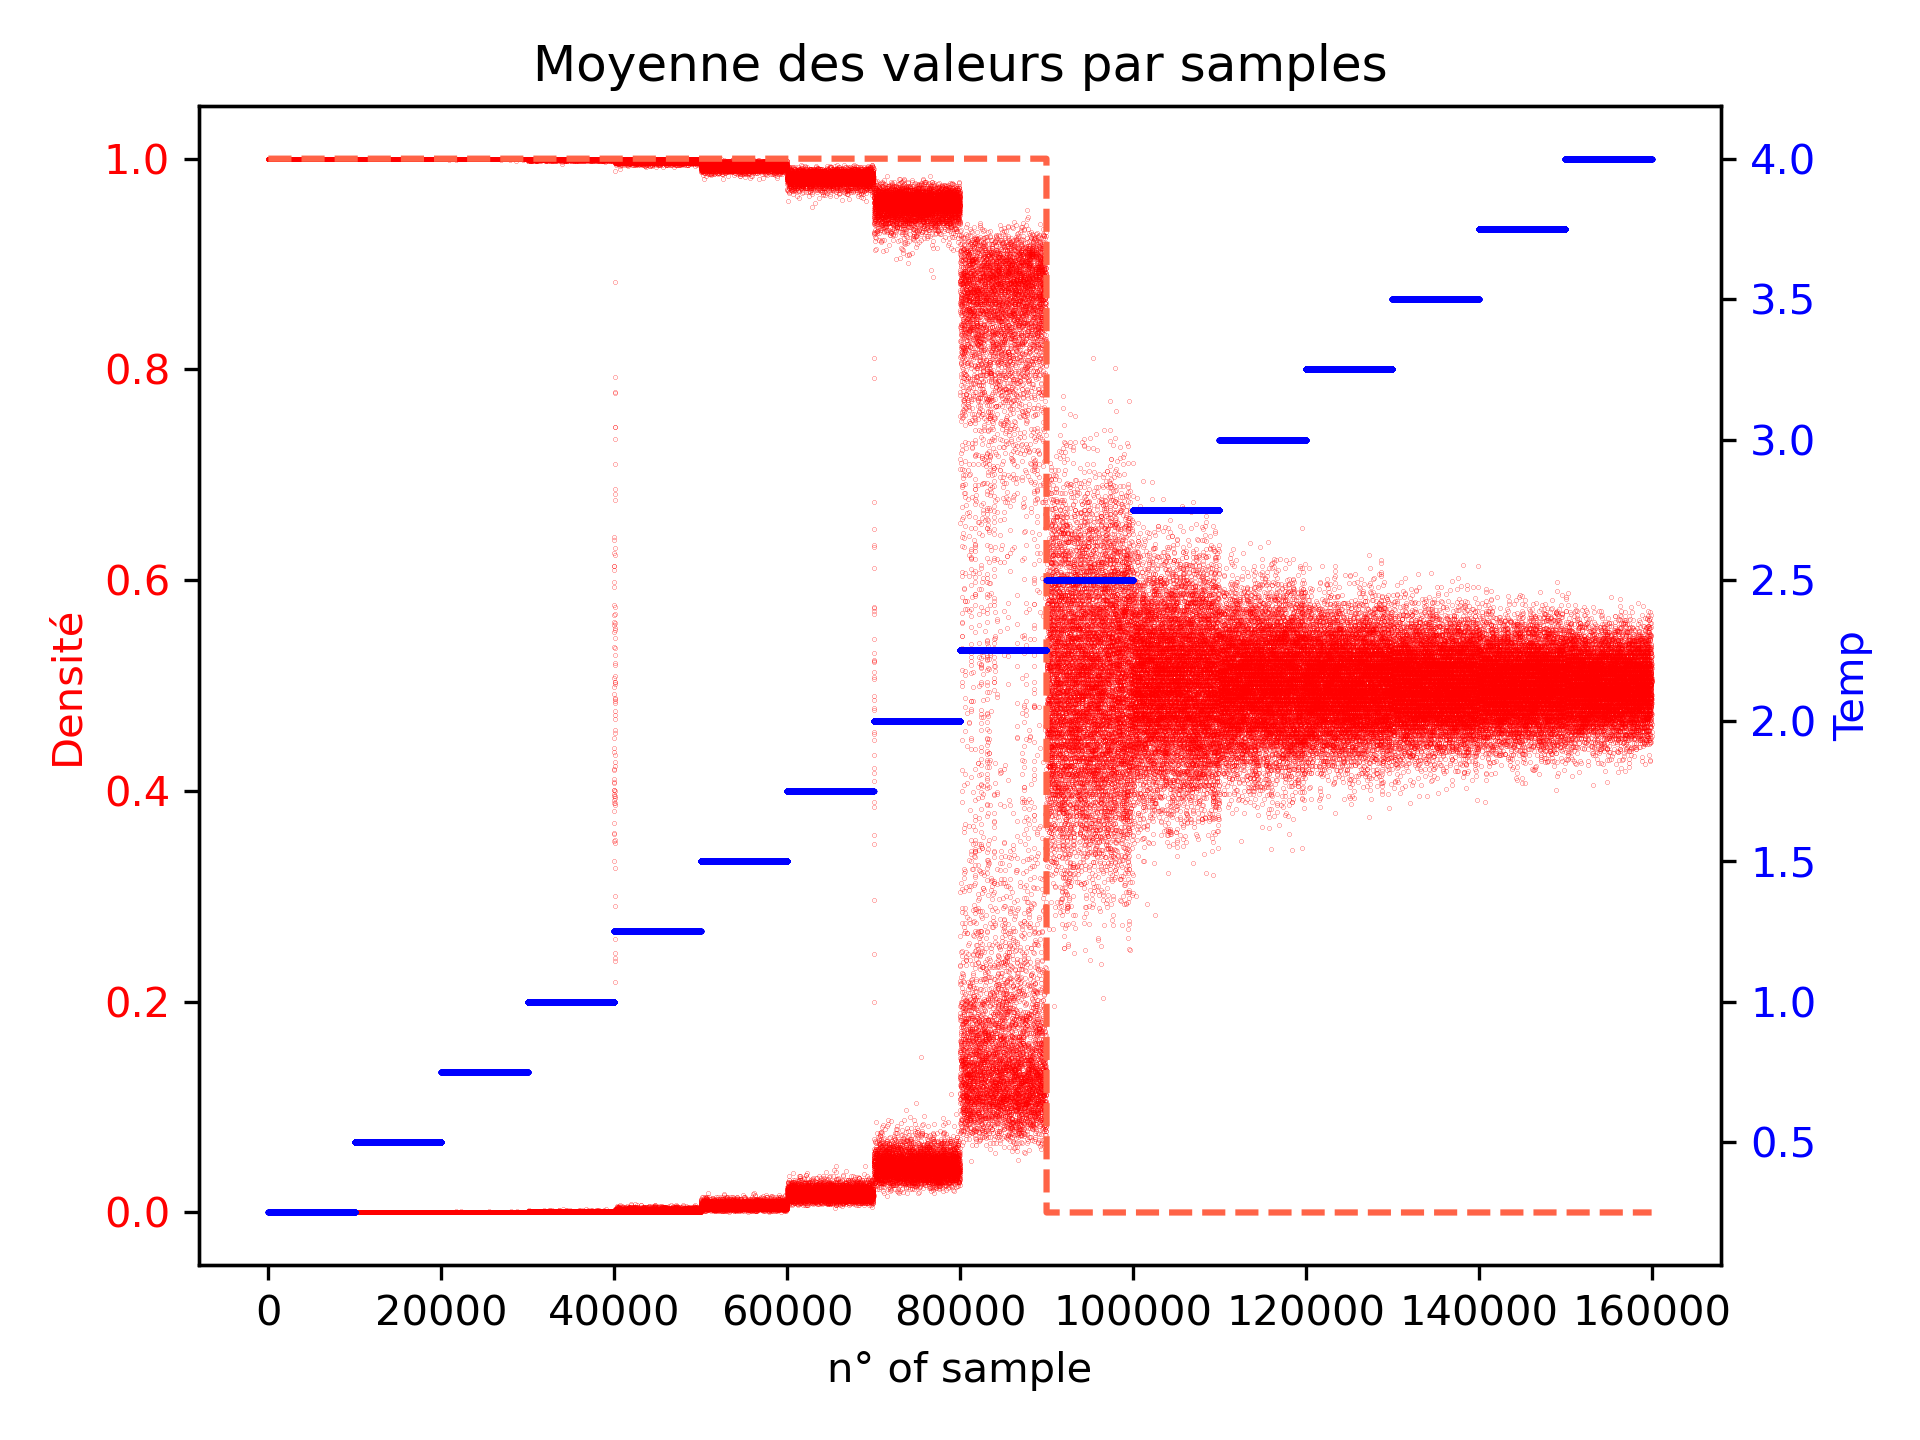
\includegraphics[width=0.95\linewidth]{./figures/raw_data.png}
		\caption{Données brutes}
		\label{fig:rawdata}
	\end{subfigure}
	\begin{subfigure}{0.5\textwidth}
		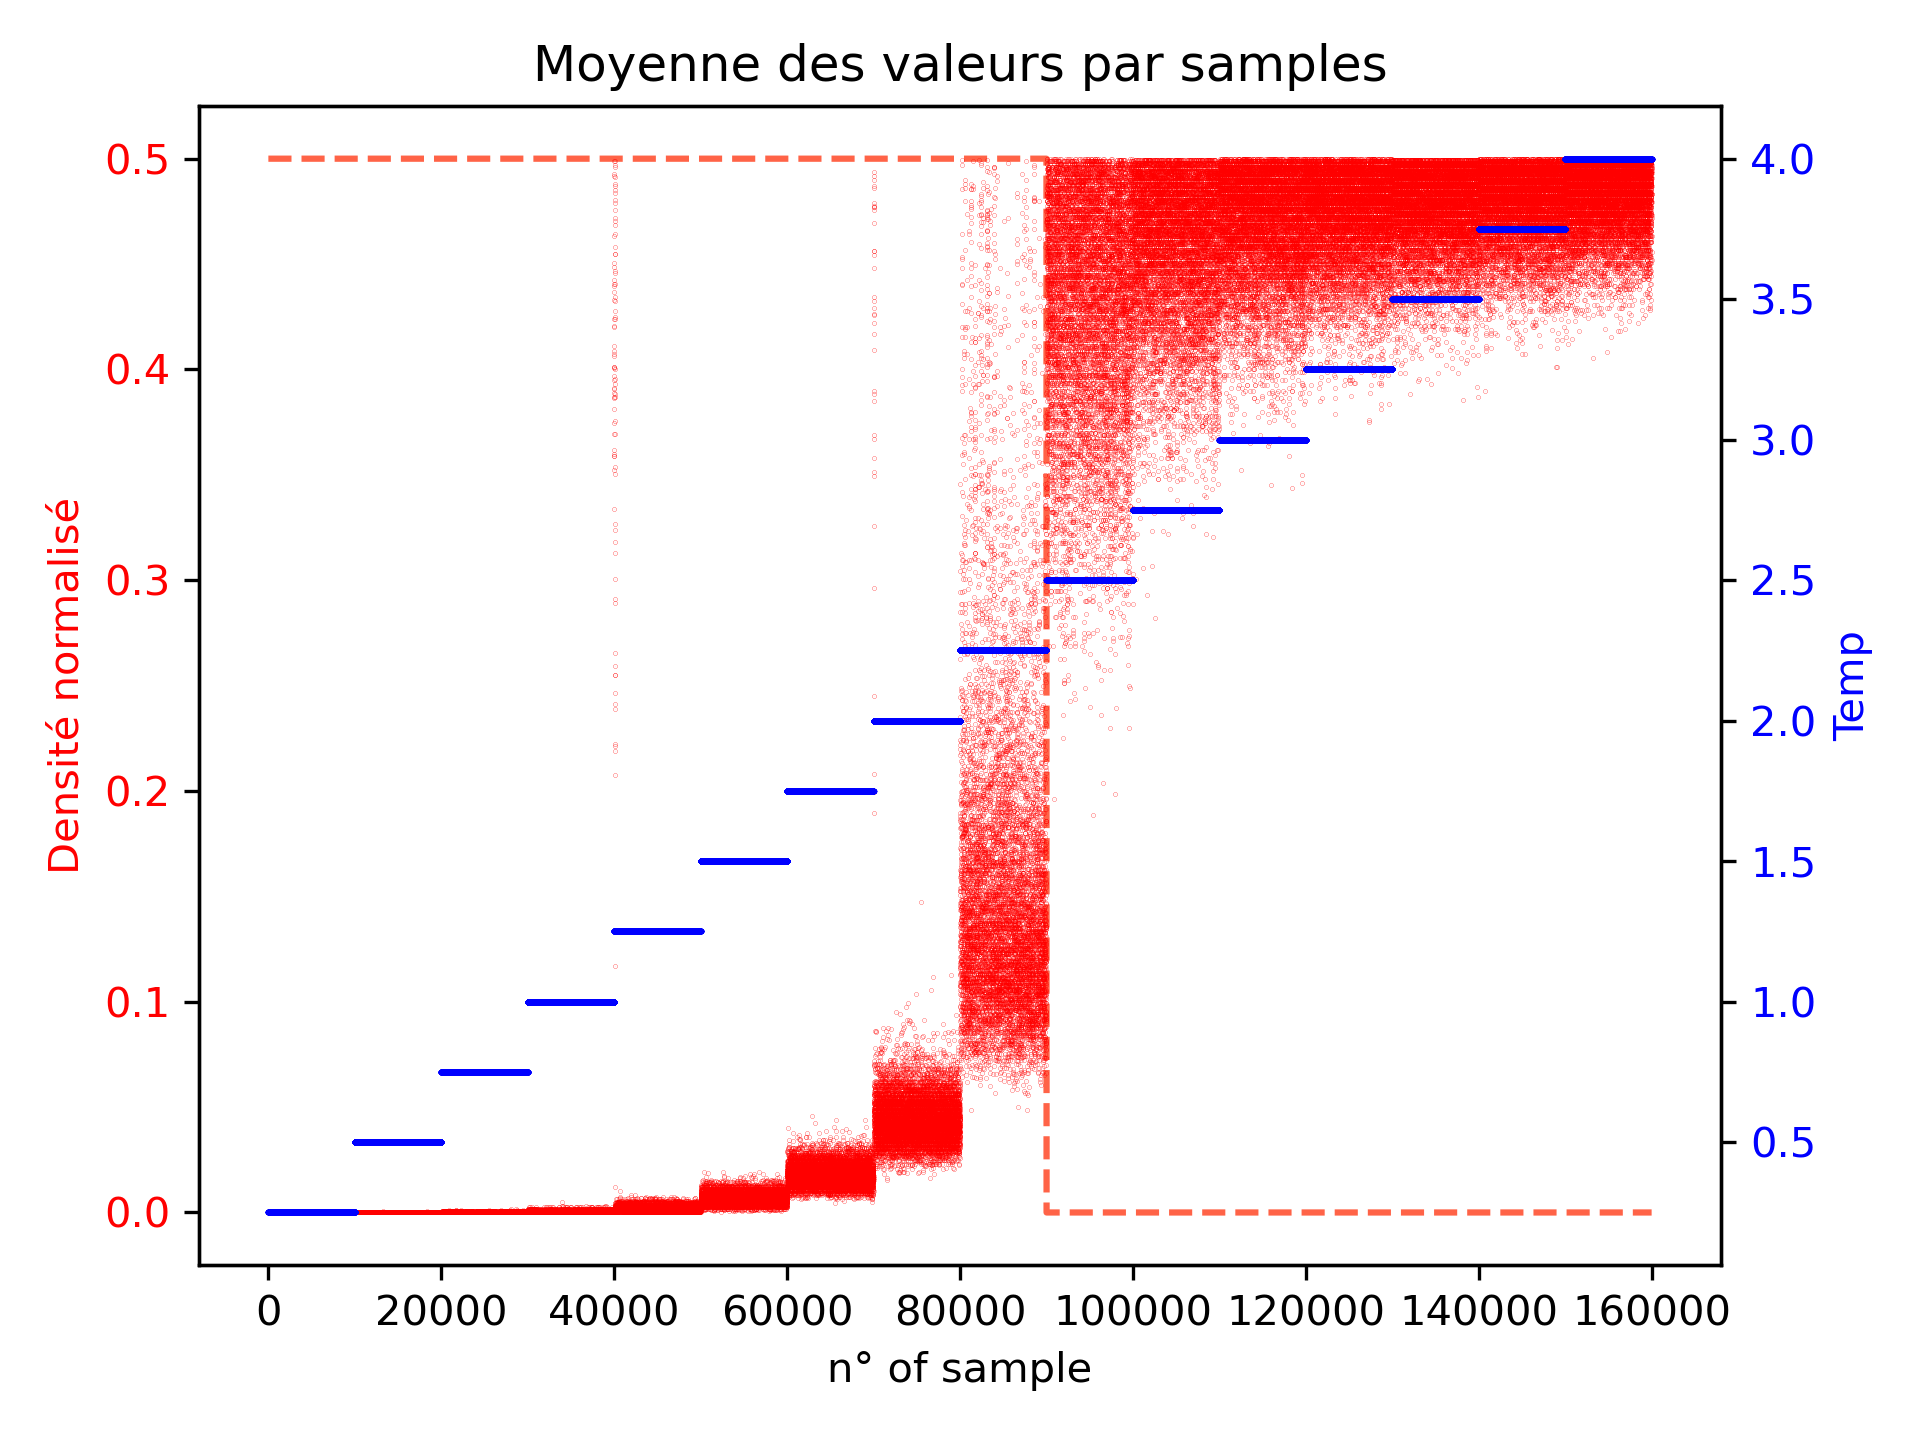
\includegraphics[width=0.95\linewidth]{./figures/sym_data.png}
		\caption{Données symétrisées}
		\label{fig:symdata}
	\end{subfigure}
	\caption{}
\end{figure}

Dans la partie suivante, nous allons entraîner certains modèles spécifiques sur la densité de spin symétrisée. Dans ce cas, nous allons aussi normaliser afin de rendre les modèles plus performants.
Pour cela, nous allons utiliser la méthode \textit{StandardScaler} de la librairie \textit{sklearn} qui permet de centrer et réduire les données. Cette méthode soustrait la moyenne et divise par l'écart-type. Ainsi, on se retrouve avec des données centrées en $0$ et de variance $1$.
Afin d'appliquer exactement la même transformation sur les données de test, nous allons créer un pipeline qui va appliquer la méthode de symétrisation puis la méthode de normalisation. Ainsi, on pourra appliquer le pipeline sur les données de test sans avoir à les modifier.
Finalement, certains modèles seront plus réceptifs à des données présentées sous forme de vecteur de taille $1600$, d'autre sous forme de matrice de taille $40 \times 40$. Pour éviter de devoir modifier les données à chaque fois, nous allons créer un pipeline qui va transformer les données en \todo{De Base, sous forme matrice ou vecteur ?} matrice si nécessaire.

\section{Modèles classiques}

\section{Réseaux de neurones}

\addcontentsline{toc}{section}{Conclusion}
\section*{Conclusion}

\end{document}
